\documentclass[graphics]{beamer}
\usepackage{xcolor}
\usepackage{graphicx}
\usepackage{verbatim}
\usepackage{wrapfig}
\useoutertheme{shadow}
%\usecolortheme{orchid}
\usecolortheme{seahorse}


% math commands
\newcommand{\be}{\begin{eqnarray}}
\newcommand{\ee}{\end{eqnarray}}
\newcommand{\beq}{\begin{equation}}
\newcommand{\eeq}{\end{equation}}
\def\simless{\mathbin{\lower 3pt\hbox
      {$\rlap{\raise 5pt\hbox{$\char'074$}}\mathchar"7218$}}}
\def\simgreat{\mathbin{\lower 3pt\hbox
      {$\rlap{\raise 5pt\hbox{$\char'076$}}\mathchar"7218$}}} %> or of order

% variables

\def\toonscale{0.45}
\def\mboxy#1{\mbox{\small #1}}

\defbeamertemplate*{title page}{customized}[1][]
{
  \usebeamerfont{title}\inserttitle\par
  \usebeamerfont{subtitle}\usebeamercolor[fg]{subtitle}\insertsubtitle\par
  \bigskip
  \usebeamerfont{author}\insertauthor\par
  \usebeamerfont{institute}\insertinstitute\par
  \usebeamerfont{date}\insertdate\par
  \usebeamercolor[fg]{titlegraphic}\inserttitlegraphic
}
\begin{comment}
\AtBeginSection[]{
  \frame{
    \frametitle{Outline}
    \tableofcontents[currentsection]
  }
}
\end{comment}



\begin{document}

%\section*{Introduction}
\section{Introduction}

\begin{comment}
  \subsection{Outline}

  \frame{
    \frametitle{Outline}
    \tableofcontents
  }
\end{comment}

  \frame{
    \frametitle{Overview}
    \begin{itemize}
      \item ARO: 46m dish
      \item Algonquin Park: remote site
      \item Dunlap project
      \item VLBI
    \end{itemize}
\vspace{-0.4in}
\hspace{1.3in}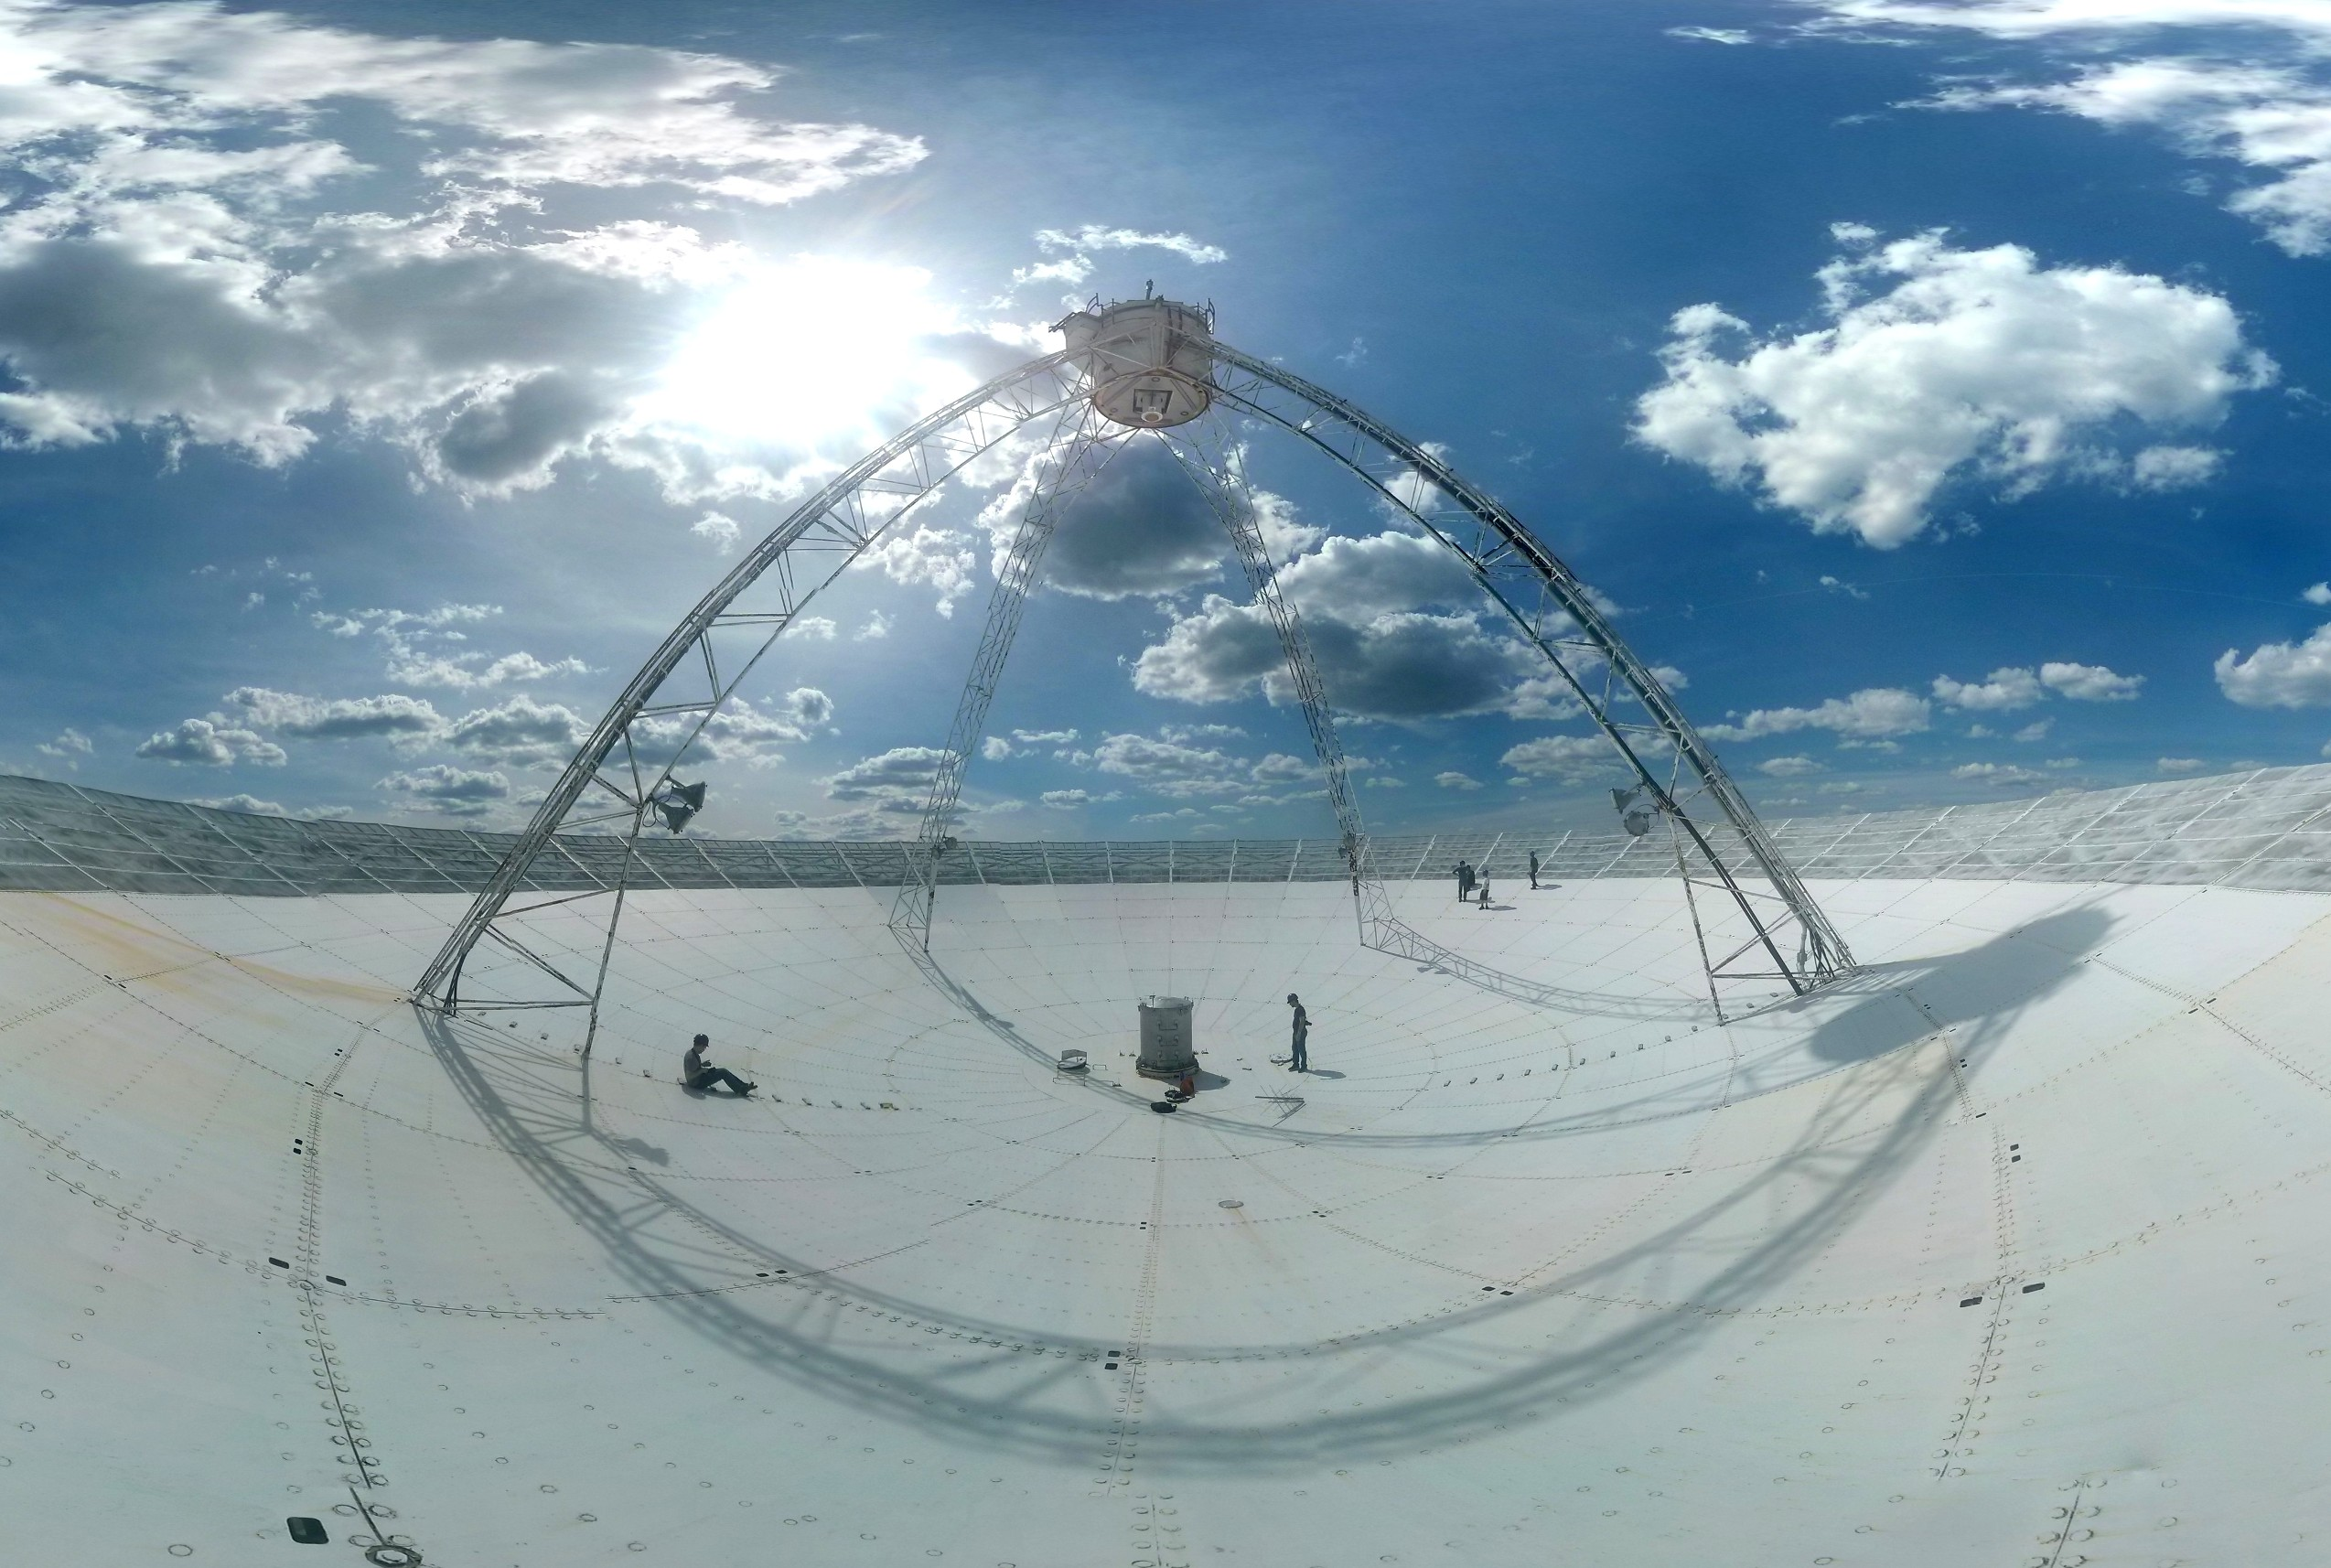
\includegraphics[width=3.2in]{Figures/PANO-20140610-155348-Phils-panorama-dish-cropped-scaled.jpg}
  }


\section{History}
 \frame{
    \frametitle{VLBI}
    \begin{itemize}
        \item April 17, 1967. First VLBI ARO-DRAO, Galt, Yen et al. 
\item IEEE Milestone:  
{\it 
VLBI combines the signals of widely separated telescopes in order to
form a single observation range.  In the experiment that was
recognized as an IEEE Milestone, the range achieved between a first
telescope at the DRAO facility in Penticton, British Columbia and a
second one in Algonquin Park, Ontario was 3,074 kilometers
}
\item the next IEEE milestones: invention of video games, LCD's, CERN, internet. 
    \end{itemize}
}

\section{Pulsars}

\frame{
    \frametitle{Pulsars}
     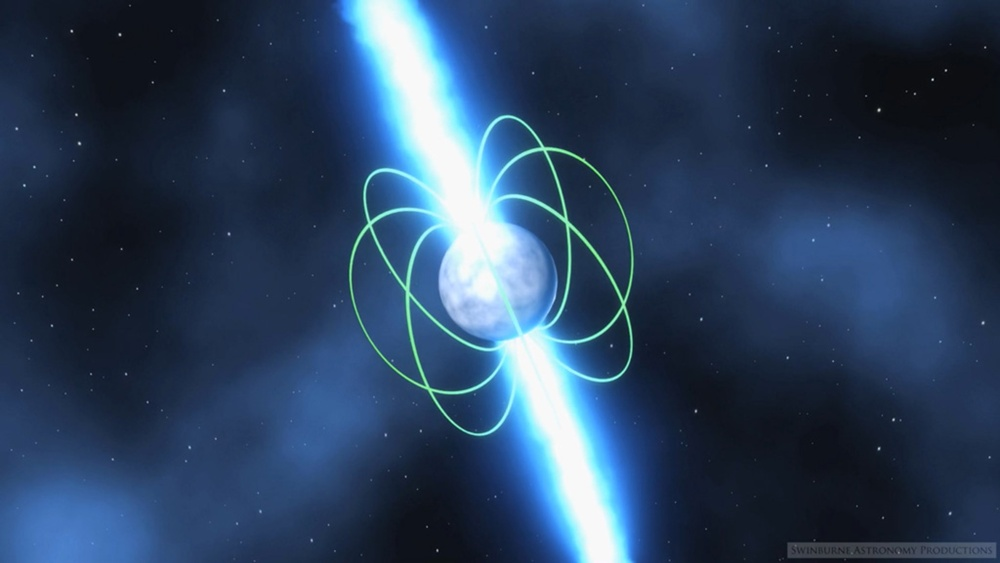
\includegraphics[width=\textwidth]{Figures/Pulsar.jpg}
{\tiny \newline 
http://www.astronomy.com/news/videos/2014/05/astronomers-harness-the-galaxys-biggest-telescope-to-make-most-precise-measurement-of-spinning-star
}
}

  \frame{
\vspace{-0.5in}
    \frametitle{Pulsar VLBI}
    \begin{itemize}
        \item brightest known radio intensity in the universe ($T_B>10^{38}$K)
        \item radar/holography imaging through ISM
        \item potential for imaging pulsar magnetosphere, ISM.
%          \vspace{-0.15in}
    \end{itemize}
\vspace{-0.1in}\hspace{.3in}
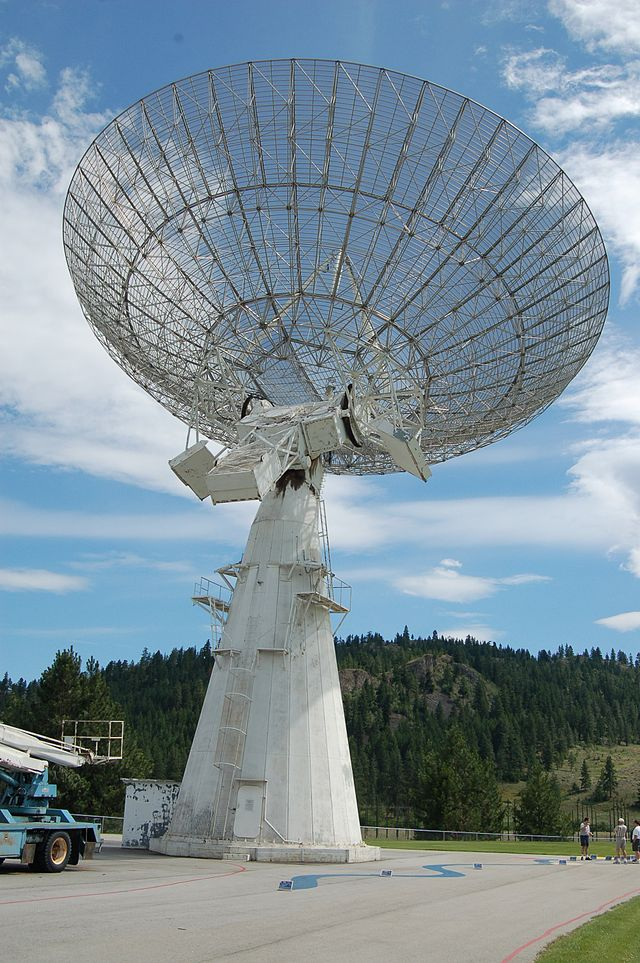
\includegraphics[width=1.2in]{Figures/DRAO_26m_dish.jpg}
\vspace{-0.5in}
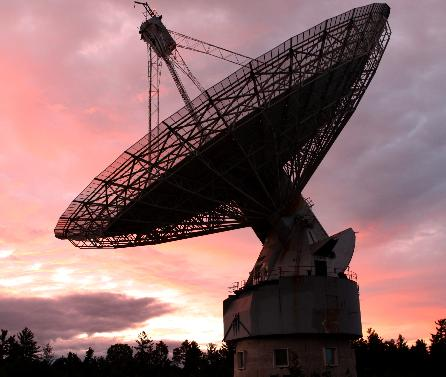
\includegraphics[width=1.9in]{Figures/IMG-7749-ARO-crop.JPG}
  }
  \frame{
\vspace{-0.5in}
    \frametitle{Canadian VLBI fringes!}
    \begin{itemize}
      \item work by Liam Connor, Robert Main
        \item crab giant pulse
        \item April 2016, ARO-DRAO
%          \vspace{-0.15in}
    \end{itemize}
\vspace{-0.1in}\hspace{.3in}
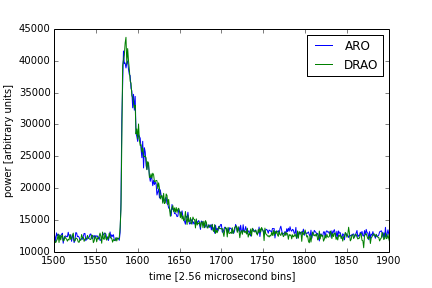
\includegraphics[width=1.9in]{Figures/ARO-DRAO-PulseComp.png}
\vspace{-0.5in}
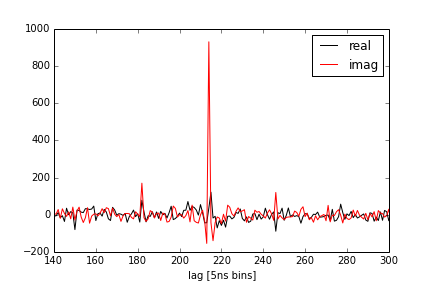
\includegraphics[width=1.9in]{Figures/ARO-DRAO-lf-zoom.png}
  }

  \frame{
    \frametitle{Projects}
    \begin{itemize}
    \item Seed funded with \$30,000 from Dunlap in 2012 
    \item Resulted in new industrial funding streams: CRD, OCE,
      SOSCIP, IBM
     \item Summer courses (399Y), workshops (CAASTRO), 
    \end{itemize}
  }

  \frame{
    \frametitle{Applications}
    \begin{itemize}
        \item so far, two pulsar Nobel prizes (on par with CMB)
        \item potential direct detection of gravitational waves
        \item precision tests of GR
        \item matter at extreme conditions
        \item probes of the ISM
        \item huge voltage datasets, currently PB.
\vspace{-0.1in}
    \end{itemize}
\vspace{-0.6in}\hspace{2.9in}
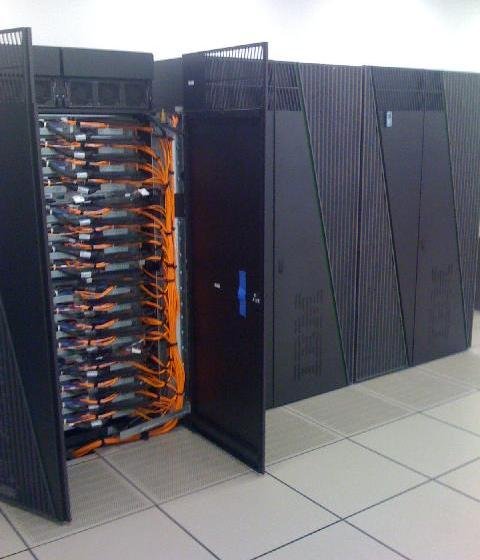
\includegraphics[width=1.5in]{Figures/BGQrack2s.jpg}
  }



  \frame{
    \frametitle{Gravitational Waves}
    \begin{itemize}
    \item Pulsar Timing Array (PTA): use pulsars as clocks
    \item sensitive to light decade GW waves: supermassive binary BH's.
    \item currently incoherent: discard pulsar phase, use only earth
      phase
    \item incoherent limitations: angular resolution $\sim 90^o$,
      impossible followup, oncoherent stochastic background?
    \item coherent PTA (Boyle+UP 2012): use distances to pulsars, resolution =
      $\lambda/D \sim 10 ly/10,000 ly \sim$ arc minute.
    \item doubles sensitivity
    \end{itemize}
  }

\frame{
    \frametitle{PTA}
%\vspace{-0.6in}\hspace{2.9in}
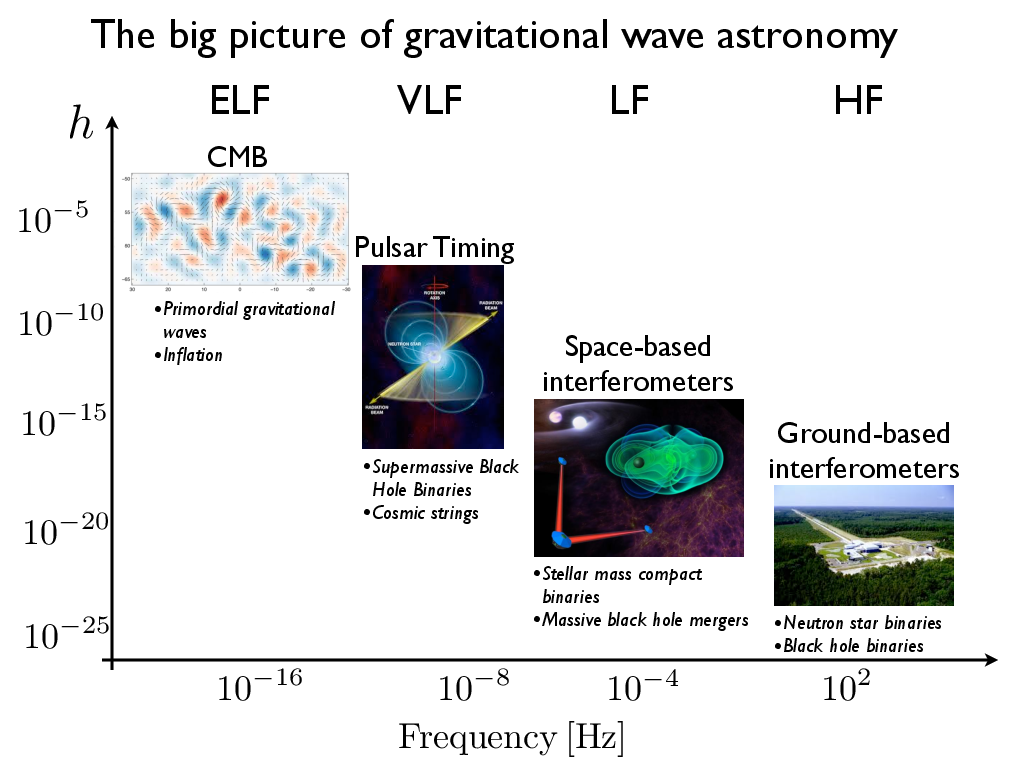
\includegraphics[width=3.8in]{Figures/GWBigPicture.png}
nanograv.org
  }


  \frame{
    \frametitle{Current Status}
    \begin{itemize}
      \item first fringes with DRAO (Penticton)
    \item new network of low frequency pulsar VLBI telescopes: Penticton, Algonquin,
      GMRT (India), LOFAR (Netherlands), MWA (Australia)
     \item new analysis techniques: Scintillometry 
    \end{itemize}
  }

\section{Summary}
  \frame{
    \frametitle{Looking forward}
    \begin{itemize}
      \item regular DRAO-ARO broadband pulsar VLBI + other networks
      \item emission structure of pulsars
      \item binary orbit parameters: potentially most massive neutron
        star 1957+20?
      \item ISM lensing: precise distances?
      \item Pulsar size measurements, equation of state?
    \end{itemize}
  }


\end{document}
